\chapter{Data and Methodology}
\label{chap:data_methodology}

This section details the data sources and methodological approaches employed in this thesis. It begins by describing the primary data source, the ICIJ Offshore Leaks Database (Section \ref{sec:3_1}), and the external datasets used for contextualization (Section \ref{sec:3_2}). Subsequently, it introduces a novel methodology utilizing agentic AI to enrich intermediary classification (Section \ref{sec:3_3}), outlines the general analytical methodologies applied (Section \ref{sec:3_4_analytical_methodologies}), and finally comments on the use of LLMs in the thesis preparation (Section \ref{sec:3_5_llms}).

\section{The ICIJ Offshore Leaks Database}
\label{sec:3_1}

\subsection{The Difficulty in }

Kejriwal \& Dang (2020) note:

\begin{quote}
"However, precisely because the collection maps out a global system, the Panama Papers also present us with a golden opportunity to study the flow of information2 between firms, individuals and intermediaries. From a scientific perspective, the Panama Papers repre- sent a complex system, with entities that range from individuals to companies, many of which serve a specific purpose based on where in the world they are based, to a variety of relationships. Studying the structural properties of this complex system using applied networks science has the potential to reveal interesting trends about how such systems operate across geographies and economies."
\end{quote}


The use of the ICIJ Offshore Leaks Database for this type of research is increasingly established. For example, Alstadsæter et al. (2019), Londoño-Vélez \& Ávila-Mahecha (2021), and Chang et al. (2023a; 2023b).

\subsection{Overview of the ICIJ Offshore Leaks Database}

Our primary dataset is the **International Consortium of Investigative Journalists (ICIJ) Offshore Leaks Database**. This publicly accessible repository is a comprehensive amalgamation of structured data meticulously extracted from several of ICIJ's landmark global investigations, most notably the Offshore Leaks (2013), Panama Papers (2016), Paradise Papers (2017/18), and Pandora Papers (2021/22). The database is substantial, cataloging information on over 810,000 offshore entities—which encompass a range of structures such as companies, trusts, and foundations—and establishing connections to more than 750,000 individuals and corporate entities. These connections span across a vast geographical landscape of over 200 countries and territories, with the underlying records covering a significant historical period, in some cases extending up to the year 2020.

\begin{figure}[htbp]
    \centering
    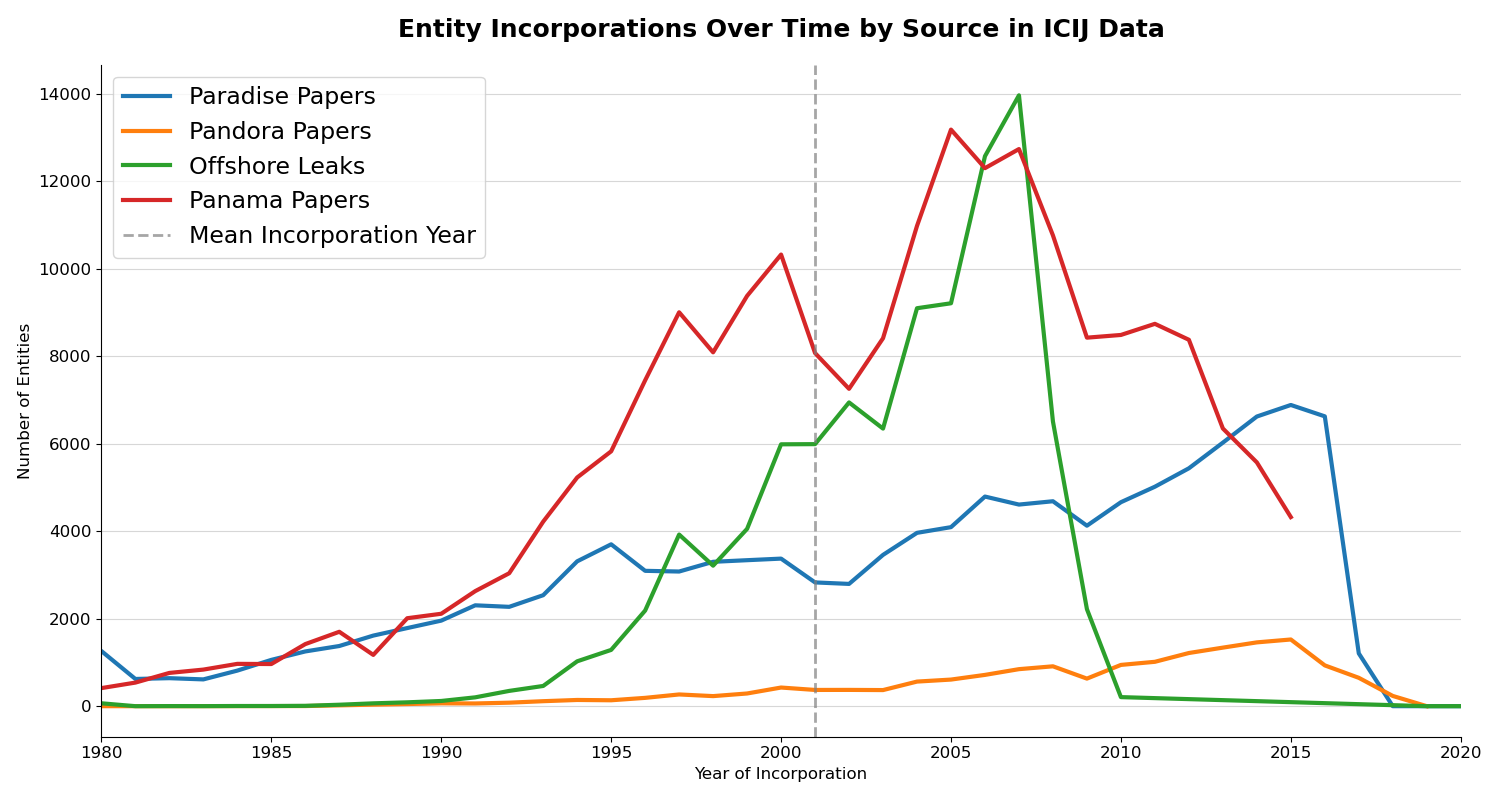
\includegraphics[width=0.8\textwidth]{Preliminary_Incorporations_over_Time.png}
    \caption{Overview of Entity Incorporations Over Time from ICIJ Data}
    \label{fig:incorporations_time}
\end{figure}

Before getting into the explanation, it's important to note, that the overview provided here is relatively cursory and focuses mostly on the attributes and feature engineering specific to this thesis. For those more familiar with network analysis, I'd strongly encourage Kejriwal \& Dang's (2020) to get a more in-depth understanding of the data in more graph-theoretical terms.

The fundamental data model leveraged by the ICIJ data is a graph database. This model is used for its ability to represent interconnected information, conceptualizing data as **nodes** (the core informational units) and **edges** (the links defining how these units are connected). For the purposes of our study, the most pertinent node types, as detailed in `icij_data_overview.md` and reflected in the input CSV files like `nodes-entities.csv`, `nodes-officers.csv`, etc., are:

*   **Entities**: These represent the diverse offshore legal structures documented in the leaks, such as Limited companies, S.A. (Société Anonyme), Inc. (Incorporated), trusts, and foundations.
*   **Officers**: This category includes individuals or, in some instances, other corporate bodies that fulfill specific roles (e.g., director, shareholder, beneficial owner, trustee, protector, nominee) within an Entity.
*   **Intermediaries**: These are the professional facilitators—typically law firms, accounting practices, banks, trust companies, or specialized middlemen—who assist clients in the establishment and ongoing management of offshore entities. They often act as the liaison with offshore service providers like Mossack Fonseca or Appleby.
*   **Addresses**: These nodes capture physical location data associated with the other node types, such as the registered office of an Entity or the business address of an Intermediary.

Relationships within this graph structure explicitly define the nature of the connections, for example, an Officer is an `officer_of` an Entity, or an Intermediary acts as an `intermediary_of` an Entity. The two primary node types of interest here are entities and, of course, intermediaries. In the data model here, intermediaries role is, with very, very few exceptions represented entirely through entities. That is, at a high level, intermediaries are `intermediary_of` entities, which are `officer_of` officers. 


\subsection{Entities}

Delving deeper into the **entities**, the information processed from source files such as `nodes-entities.csv` and `relationships.csv` provides a rich set of attributes for each. Key data points include the entity's registered `name`, its `jurisdiction` of incorporation (which I standardize to ISO3 country codes for consistent geographical analysis), and the `country_codes` associated with its operational activities or linked addresses (these are often distinct from its legal jurisdiction of incorporation). Further attributes encompass the `incorporation_date`, its operational `status` (e.g., Active, Struck Off, Dissolved), and its specific `entity_type` (e.g., Standard International Company, Trust, Business Company Limited by Shares). A particularly significant feature we derive for each entity, as processed in is the `bearer_count`. This metric quantifies the number of associated officers explicitly identified as "Bearer" or its linguistic equivalents (e.g., "THE BEARER," "EL PORTADOR"), which we standardize from variations found in `officers_df`. The presence of bearer instruments, as highlighted by Harrington (2016), is a critical indicator of mechanisms used to obscure true beneficial ownership, as ownership follows the physical possession of the share certificate rather than being registered.

\subsection{Intermediaries and Feature Engineering}

For **intermediaries**, whose foundational data is drawn from `nodes-intermediaries.csv`. Beyond basic identifying information such as their `name` and the `countries` associated with their operational addresses, we calculate their `degree`, which represents the total number of distinct entities they are connected to within the ICIJ network. More extensively, we construct several aggregated metrics that characterize each intermediary based on the collective properties of the entities they service. Because our primary interest is in intermediaries, we aggregate information up at the intermediary-level about the entities they're connected to. Graphs as a data model are incredibly good for being able to contain difficult, interrelated data, but also incredibly difficult to work with, so aggregating information up in key-value pairs. 

For every intermediary, we generate:
*   `country_counts`: A dictionary detailing the frequency of entities they are connected to, grouped by the `country_codes` associated with those entities (reflecting where the entities have operational links).
*   `jurisdiction_counts`: A dictionary detailing the frequency of entities they are connected to, grouped by the `jurisdiction` in which those entities are incorporated.
*   `regime_counts`: A dictionary detailing the frequency of entities they are connected to, grouped by the political regime type (e.g., Liberal Democracy, Closed Autocracy) of the entities' associated `country_codes`.
*   `legal_tech_counts`: A dictionary detailing the frequency of entities they are connected to, grouped by the predominant types of "legal technologies" (e.g., Banking, Corporate, Dual-Purpose) prevalent in the entities' jurisdictions of incorporation at the time of their formation.

Furthermore, we quantify for each intermediary the number of entities they are connected to that have `bearers_connected` (i.e., entities with a `bearer_count` > 0) and calculate the `bearer_share`, representing the proportion of their serviced entities that utilize bearer instruments. To measure the diversity of their client entity portfolio across these dimensions, we also compute normalized entropy scores (more on that later in this section): `country_entropy`, `jurisdiction_entropy`, `regime_entropy`, and `legal_tech_entropy`. These scores provide a standardized measure of how dispersed or concentrated an intermediary's entity connections are across different countries, jurisdictions, regime types, and legal technology environments.

\section{External Data Sources}
\label{sec:3_2}

The following external data sources are used to connect with and enrich the ICIJ data:
\begin{itemize}
    \item \textbf{Laffitte Legal Technologies Data (HTHD)}: This dataset (Laffitte, 2024) is used for connecting historical legal framework changes to entities and their structuring.
    \item \textbf{VDem (Varieties of Democracy) Data}: This provides country-level variables for the jurisdictions associated with entities and intermediaries.
    \item \textbf{Intermediary Type Enrichment}: As detailed in Section \ref{sec:3_3}, an agentic AI approach is used to classify intermediaries based on scraped data.
\end{itemize}

At the country(/jurisdiction)-level we use the Varieties of Democracy (VDem) data for information on the regime type, and Sebastien Laffitte's (2024) Historical Tax Havens Database dataset (HTHD) developed/collated for his thesis, with information on the legal technologies in the jurisdictions. 

1.  The **Varieties of Democracy (VDem) Project data** (specifically `vdem_core.csv`): We utilize the `v2x_regime` variable from VDem's comprehensive dataset to enrich our entity data. By matching an entity's associated `country_codes` and its `incorporation_year` with the VDem data, we assign a political regime classification to each entity. This entity-level regime information is then aggregated to construct the `regime_counts` at the intermediary level, providing insight into the political environments linked to an intermediary's clientele.
2.  **Laffitte's (2024) "The Market for Tax Havens" dataset** (specifically `HTHD.csv`): This dataset offers a historical perspective on the "offshore legal architecture" of various jurisdictions, detailing their adoption of different "legal technologies" such as IBC laws, trust legislation, or banking secrecy provisions. We merge this dataset onto our entity data by matching the entity's `jurisdiction` of incorporation and its `incorporation_year`. This allows us to identify the specific legal technologies (e.g., "Banking," "Corporate," "Dual-Purpose," "Personal") active in an entity's jurisdiction at its time of incorporation. This entity-level characterization is subsequently aggregated to create the `legal_tech_counts` at the intermediary level, reflecting the types of legal environments their serviced entities operate within.

The aggregation process to derive `jurisdiction_counts` and `regime_counts` (and similarly `country_counts` and `legal_tech_counts`) at the intermediary level is a natural consequence of our data structure. Once each entity connected to an intermediary is characterized by its jurisdiction, associated country regime, or jurisdictional legal technology, we simply count the occurrences of these characteristics across all entities linked to a given intermediary.

Directly at the Intermediaries-level, we also enrich a subset of intermediaries with information on the specific "type" derived from the typology in the EU(2017) paper. 

The core idea is to use an AI agent loop to automate the process of gathering information about and classifying the intermediaries listed in the ICIJ data. The basic workflow is illustrated in Figure \ref{fig:agent_loop_placeholder}.

\begin{figure}[htbp]
    \centering
    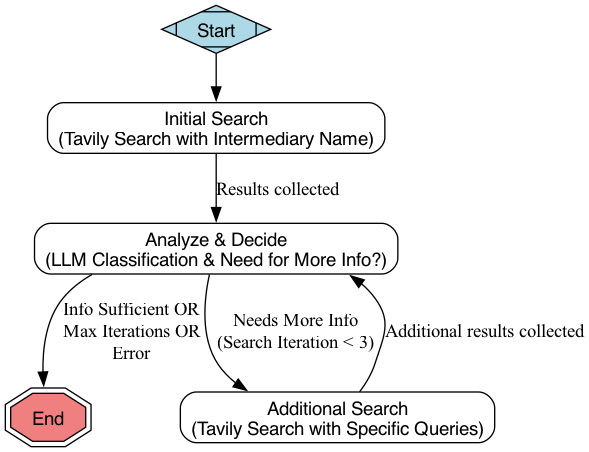
\includegraphics[width=0.8\textwidth]{Methods_Agent_Graph.png} % Assuming you have agent_graph.png
    \caption{Agent Setup for Intermediary Classification}
    \label{fig:agent_loop_placeholder}
\end{figure}

In brief, the process involves an AI agent orchestrating online searches for each intermediary identified in the ICIJ data. It begins with generic searches, reads and interprets the initial results, and then formulates more specific search queries based on the information discovered or identified as lacking. This iterative process involves up to three search queries per intermediary, scouring the top 15 most relevant web results identified through query-result embedding similarity using the Tavily Search API (though the tool is relatively generic and its specific choice is not critical to the methodology). This effectively replaces the time-consuming need for manual searching of the intermediaries.

Based on the information gathered, the AI agent then classifies the intermediary according to the EU (2017) typology (Tax Expert, Legal Expert, Administrator, Investment Advisor), adding a few additional relevant fields (e.g., specific job title). Crucially, the agent also provides a confidence score for its classification judgment, allowing for filtering or weighting in subsequent analyses.


There are a few obvious limitations associated with this approach that warrant discussion:
\begin{itemize}
    \item The "Small Spiders" Problem. Kimberly Kay Hoang notes of one of the ultra-wealthy board directors she interviews, that despite the entities he was behind were revealed in the Panama Papers, nothing traces back to him. Instead, a group of "fall guys", as she terms them, are the ones that fall victim to the public's search-light. Those that have public profiles skew the bias towards the less illict people involved even stronger.
    \item Temporal Misalignment: A primary concern is that all online searches are conducted based on information available today, whereas the ICIJ data pertains to activities that may have occurred years or even decades prior. This introduces two potential issues:
    \begin{enumerate}
        \item The process might be biased towards identifying intermediaries who are still active or have a significant online presence currently.
        \item It implicitly assumes that the role an intermediary plays today (as reflected online) is equivalent to the role they played at the time relevant to the ICIJ data.
    \end{enumerate}
\end{itemize}

Addressing the Limitations: While these issues are real, they are not prohibitive for their use in this thesis.
\begin{enumerate}
    \item Regarding the first point (bias towards current intermediaries), this primarily impacts the coverage or statistical power of the classification – we may only be able to confidently classify a subset (e.g., 50\%) of all intermediaries. This is acceptable, provided the unclassifiable intermediaries are not systematically different in ways that correlate with the research questions. The issue becomes problematic only if there is a systematic bias in identifiability across types (e.g., if it is inherently much harder to find information online about legal experts compared to tax experts due to differing needs for discretion or public visibility). The significant threat here is the bias in who provides public information - it will only be the intermediaries whose activities are not inherently illegal. A bias towards, in a sense, the least dangerous intermediaries as those being revealed.
    \item Regarding the second point (role stability), the assumption that roles remain consistent is arguably less problematic. Given the highly specialized nature of functions like tax advisory, legal structuring, administration, and investment management within the offshore context, and the considerable barriers to entry (qualifications, reputation, networks) for each, frequent switching between these core roles by individuals or firms seems relatively unlikely.

\section{Analytical Methodologies}
\label{sec:3_3_analytical_methodologies}

This section outlines the core analytical techniques applied to the processed data. This includes concepts from network theory for characterizing the structure of the ICIJ data, unsupervised learning methods for pattern discovery, and statistical tests for assessing the significance of findings.

\subsection{Network Analysis Concepts}
\label{subsec:network_theory_concepts}

The analysis of the ICIJ data leverages several concepts from network theory to understand its structural properties. As highlighted by previous research (e.g., Kejriwal \& Dang, 2020; Chang et al., 2023a, 2023b), network science provides a powerful lens for this type of inquiry. Key concepts employed include:

\begin{itemize}
    \item \textbf{Overall data model}: As described in Section \ref{subsec:icij_structure}, considering the multi-modal nature of the graph and projections thereof.
    \item \textbf{Centrality scores and in-betweenness}: To identify key actors and relational importance within the network.
    \item \textbf{Louvain community detection}: To uncover clusters or communities of closely related nodes.
    \item \textbf{Power-law distribution}: To examine the distribution of node degrees and other network properties.
    \item \textbf{Density of a graph}: To measure the general level of connectedness in the network or its components.
    \item \textbf{(Entropy)}: As a measure of network information or randomness, where applicable.
\end{itemize}

\subsection{Unsupervised Learning and Association Analysis}
\label{subsec:unsupervised_learning}

To discover patterns and relationships within the data without pre-defined target labels, unsupervised learning techniques are employed, with a particular focus on association analysis.

\begin{itemize}
    \item This approach relies on a \textbf{non-parametric notion} of pattern discovery.
    \item It aims at \textbf{discovering patterns of high density} or co-occurrence.
    \item \textbf{Lift scores} will be used to quantify the strength of associations found, indicating how much more likely two items (e.g., use of a specific jurisdiction and a type of intermediary) are to appear together than expected by chance.
\end{itemize}

\subsection{Testing Significance of Results}
\label{subsec:significance_testing}
To ensure the robustness of the findings, appropriate statistical tests are utilized:
\begin{itemize}
    \item \textbf{Fisher's exact test}: Employed where applicable, particularly for categorical data and contingency tables. This is ideal for association analysis results and for dummy variables, such as whether entities are connected to bearer instruments.
    \item \textbf{Mann-Whitney U test}: A non-parametric test used for comparing continuous variables between two independent groups when the data is not normally distributed.
    \item \textbf{Two-sample Kolmogorov-Smirnov test}: Used for comparing the distributions of continuous variables from two samples, again a non-parametric choice.
\end{itemize}

\subsection{Multiple Hypothesis Testing}
\label{subsec:multiple_hypothesis_testing}
Given that this research involves exploring multiple patterns and relationships, it is crucial to address the issue of multiple hypothesis testing.
\begin{itemize}
    \item The conventional Type I error rate of 5\% ($p < 0.05$) can become inflated when multiple tests are performed, leading to a higher chance of false positives.
    \item The \textbf{Bonferroni correction} is considered, although it is known for being highly conservative.
    \item The \textbf{Benjamini-Hochberg procedure} may be a more suitable alternative to control the False Discovery Rate (FDR), offering a better balance between power and error control. However, given the exploratory nature of this work, which can be likened to a data mining exercise, a conservative approach (like Bonferroni) might be preferred to minimize false positives over maximizing statistical power. The choice of method will be justified based on the specific context of the analyses.
\end{itemize}

\section{Use of LLMs in the Broader Paper}
\label{sec:3_5_llms}

LLMs have also been used to polish the text of this thesis and used for idea generation.

Used Google Gemini models mainly.
\begin{itemize}
    \item gemini-2.5-pro-preview-05-06
    \item gemini-2.5-pro-experimental-03-25
    \item gemini-2.5-flash-experimental-04-17
\end{itemize}

Quick edits frequently made using Claude's 3.7 Sonnet model.



